\section{Discussion}\label{sec:discussion}
In this section we discuss the different features of the model, problems when computing the model,
limits of the model and ways of improving the model that we thought of when we went into more
details of the model and started to simulate it.

\subsection{Limitations of the model}

There are several limitations the model that we encountered when we started analyse and simulate the
model. In this section we discuss some relevant limitations of the model that we thought of.

The flexibility of the model in the sence that which situations it could model and some limitations
of the agents and their awareness of the environment.
E. g. (Comparison article) some people fall in panic situations and become obstacles for other people,
which is not a feature this model deals with. In our model none of the agents fall and become an obstacle force
other agents as would be seen in real life panic situations.

Another flaw in the model is that the agents do not have way finding, which mean that they can not escape
a more complex environment with a lot of rooms and corridors. As it is now we can only simulate simple
cases as the squared room and the corridor.
An improvement of the model would then be to implement way finding for the agents, so that they can manoeuvre
around in other more complex cases then the ones we have.

In other models as the HiDAC, agents can share information about the environment, such that the agents have a better
idea of where the exit is/are (Comparison article). In a real panic situation you would expect people to communicate when
evacuation a building.

Other models take into account herding behavior between the agents \cite{helbing00}, so that some people have tendency to
follow other agents, while other agents have a tendency to go their own way, and by doing so explore the environment
for possible exits.

As the model is now there is no friction between the agents, so that agents that have higher velocity than
the ones standing in their path, can slide in between slower moving agents in front of them, without them slowing
down when they slide by. In real case scenario people would not slip by that easily since the friction between
the people would slow them down.
Without friction between agents there would be less clogging in front of doors, and the time it takes the agents
to exit a room would be less than the time expected. Thus the validation of the would not be as good as if there
would be friction between the agents.

At the moment we can not simulate a case where the visibility is very low. The agents have a way point to follow,
but if the visibility only is 1 meter, e. g. in a smoke filled room, the agents would not have way point to follow,
and hence round around with out purpose. Here the tangential forces would also help the agent to find the exit,
but navigation through the tangential force from the walls.

\subsection{Discussion on walls in special cases.}\label{wallEndpoints}
The wall is created as a vector. The repulsive force vector is perpendicular to the wall 
vector and has a direction directly towards the pedestrian $\alpha$.

In the general case of the repulsive force on a pedestrian, $\alpha$, from a wall 
nearby is given as a function of the vector from the nearest point. This point we 
calculate by finding the point that makes the vector form $\alpha$ to the wall be 
perpendicular to to vector that is the wall. In some cases though the point will not 
be on the wall it self. This of course makes no sense since you would then be 
repulsed by a non existing part of the wall meaning that you would avoid free 
areas. In this case you would have to use the end point of the wall. But doing this 
can make some unrealistic behaviour as well, if the walls have the right composition. 

Let's start out by looking at a case with no problem. A case with no problems is a 
room where the angles between the walls is less than $180^o$, i.e. a squared room 
where they are $90^o$. For a pedestrian close to the corner between two walls, you 
would calculate the repulsive force from both of the walls. This you do in order 
for the pedestrian to avoid going through either one of the walls. When you do 
this you get a force directly away from each of the walls. This clearly makes 
sense and there is no problem in doing so.

The case where the angle between two walls is greater than $180^o$ could on the 
other hand give some problems if not handled correctly. The case is sketched in 
figure \ref{fig:wallcase}. Here the are 3 different areas that a pedestrian $\alpha$ 
can be in. The area A where $\alpha$ is only perpendicular to wall $1$, in area B, 
$\alpha$ will not be perpendicular to any of the walls and in C he will be only 
perpendicular to wall 2. If a pedestrian is in area B then we would calculate the 
forces from the end point of the walls. This will be from the point where the two 
walls meet. This will give you a double repulsion from one point and that 
doesn't make sense. Also when you are in are A or C you would get a repulsive force 
from a second wall you would be of no risk of going into and in many situations 
couldn't see because the first wall is blocking the sight. This of course doesn't 
make any sense either. So the way that we handle this situation is the following. 
When the angle between the walls is greater than $180^o$, from a pedestrian $\alpha$ 
point of view, you should look at the two walls as one, in the way that you will 
only calculate one force from the walls. In area A or C only the closest point 
on the closest wall should affect you. In the case of $\alpha$ being in area B 
the walls themselves doesn't matter, only the vector going from the conjoint 
point of the walls to $\alpha$, should affect and only one time. Doing this, 
there should be no unrealistic scenarios concerning wall junctions and walls 
with more than 180 degrees between them. But this could create and undesired 
behaviour at doors of other objects created with free end points.

\begin{figure}[ht]
\centering
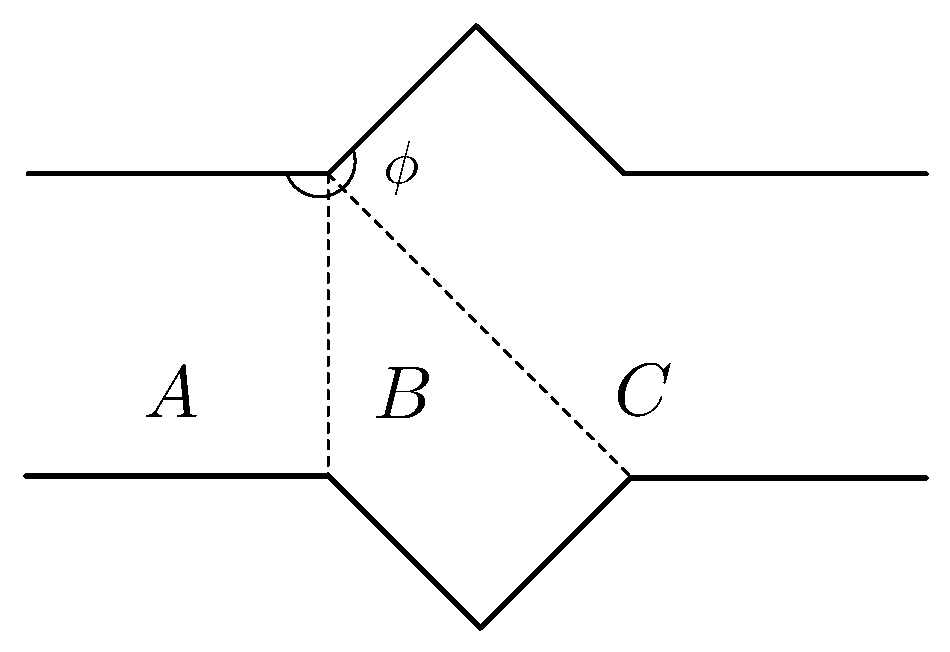
\includegraphics[scale=0.45]{Figures/WallCase.pdf} 
\caption{}\label{fig:wallcase}
\end{figure}

\subsection{The force at doorways}
We encountered a problem when dealing with doors. The problem arises because 
the door is constructed by two free endpoints and pedestrians feel a repulsion 
force from these points according to section \ref{wallEndpoints}. This means 
that a pedestrians trying to exit through the door will feel a repulsive force 
from the walls which prevent him from walking through the door. The second he 
passes through the door he will be pushed forward and accelerate which is unwanted 
behaviour. This we resolved by removing the force from free endpoint when:

\begin{equation}
\| y - w \| > R
\end{equation}

This creates what we could call a "non repulsion zone" see figure(Mikkel Lav Tegning!).
In rare cases it could happen that a pedestrian is trying to exit the room and he feels 
no repulsion because he is in the "non repulsive zone", he is then pushed sideways out 
of the "non repulsion zone" and suddenly he will feel a great repulsive force because 
he first "discovers" it when he is very close to the wall see figure(Mikkel Lav Tegning!).

\subsection{The repulsive force between agents in $ \Re ^{3}$}
From the given formula for calculating the repulsive force between agents in the 
description of the model, the part calculating the force to keep the personal space 
can be omitted when the agents are rather close to each other, then the calculation 
can be reduced as Equation (\ref{eq:re}).

\begin{equation}\label{eq:re}
\overrightarrow{f_{\alpha\beta}}(t) = A_{\alpha}^{2} exp\left[ \frac{r_{\alpha\beta} - d_{\alpha}\beta}{B_{\alpha}^{2}}\right]  \overrightarrow{n_{\alpha\beta}}
\end{equation}

Taking the norms of both sides of Equation (\ref{eq:re}), we can draw the relation 
between the value of $\overrightarrow{f_{\alpha\beta}}(t)$ and $d_{\alpha \beta}$, 
as in Figure (\ref{fig:physicalinteraction})
\\
\begin{figure}
\centering
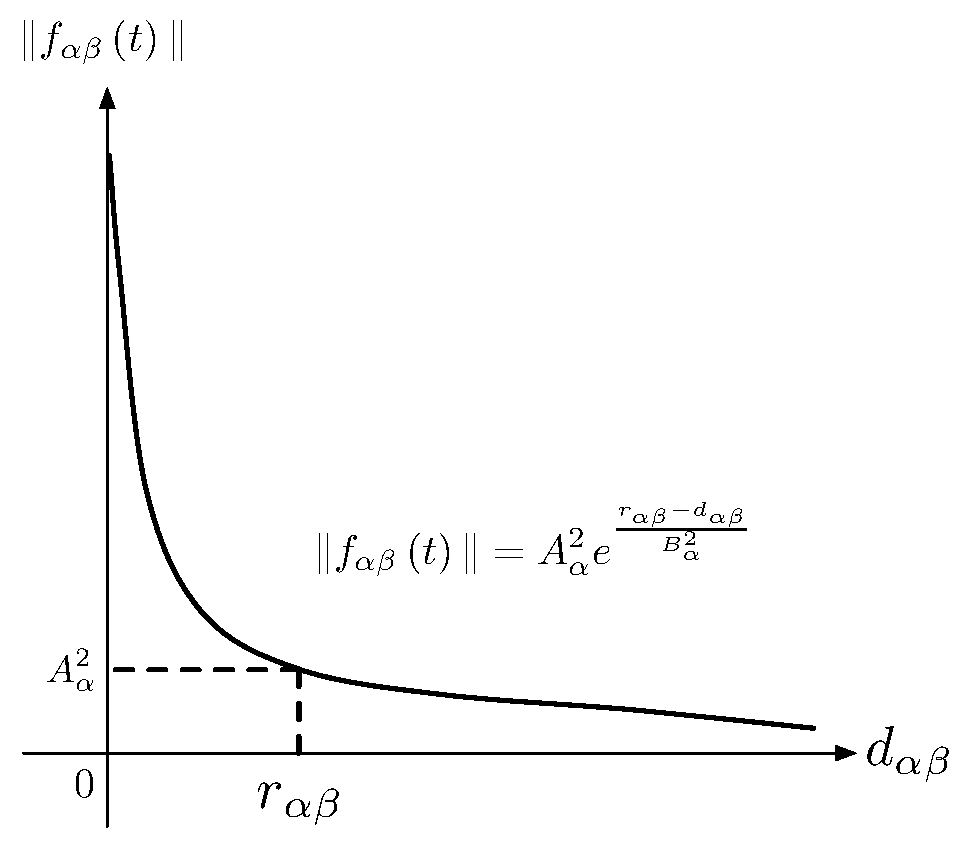
\includegraphics[scale=0.45]{Figures/physicalinteraction.pdf} 
\caption{The function about the interaction force $\vec{f_{\alpha\beta}}(t)$ and the distance between two agents
$d_{\alpha\beta}$ }\label{fig:physicalinteraction}
\end{figure}

There is one intersection of the graph and the axis $ \left( 0, A_{\alpha}^{2} exp\left( \frac{r_{\alpha\beta} }{B_{\alpha}^{2}}\right)  \right) $. 
If put into the constants, we will be able to get a maximum value of $ f_{\alpha\beta}(t) $, 
since the distance between agents cannot be negative. Here we set $ A_{\alpha}^{2} = 3 m/s^{2} $, 
$ r_{\alpha\beta} = 0.6 m $, and $ B_{\alpha}^{2} = 0.2 m $, so $ f_{\alpha\beta}(t)^{max} \doteq 60 m/s^{2} $, 
which is about six times the gravitational acceleration and represents a rather 
large force between agents (as large as six person's weight).

However, we notice that the effective part of the force calculated above is only the horizontal 
component that enables the agent to move horizontally in the plane where we do the simulation, 
but the reality is that the agents sometimes are also able to move vertically, for example, 
by stepping upon other people when they cannot take the pushing force from the surrounding agents. 
When that happens, the horizontal component of the repulsive force becomes smaller even if 
$d_{\alpha\beta}$ is kept the same.	
Therefore, a qualitative modification of dependence between $ f_{\alpha\beta}(t) $ 
and $ d_{\alpha\beta} $ could be:

\begin{figure}[hb]   
\centering
    {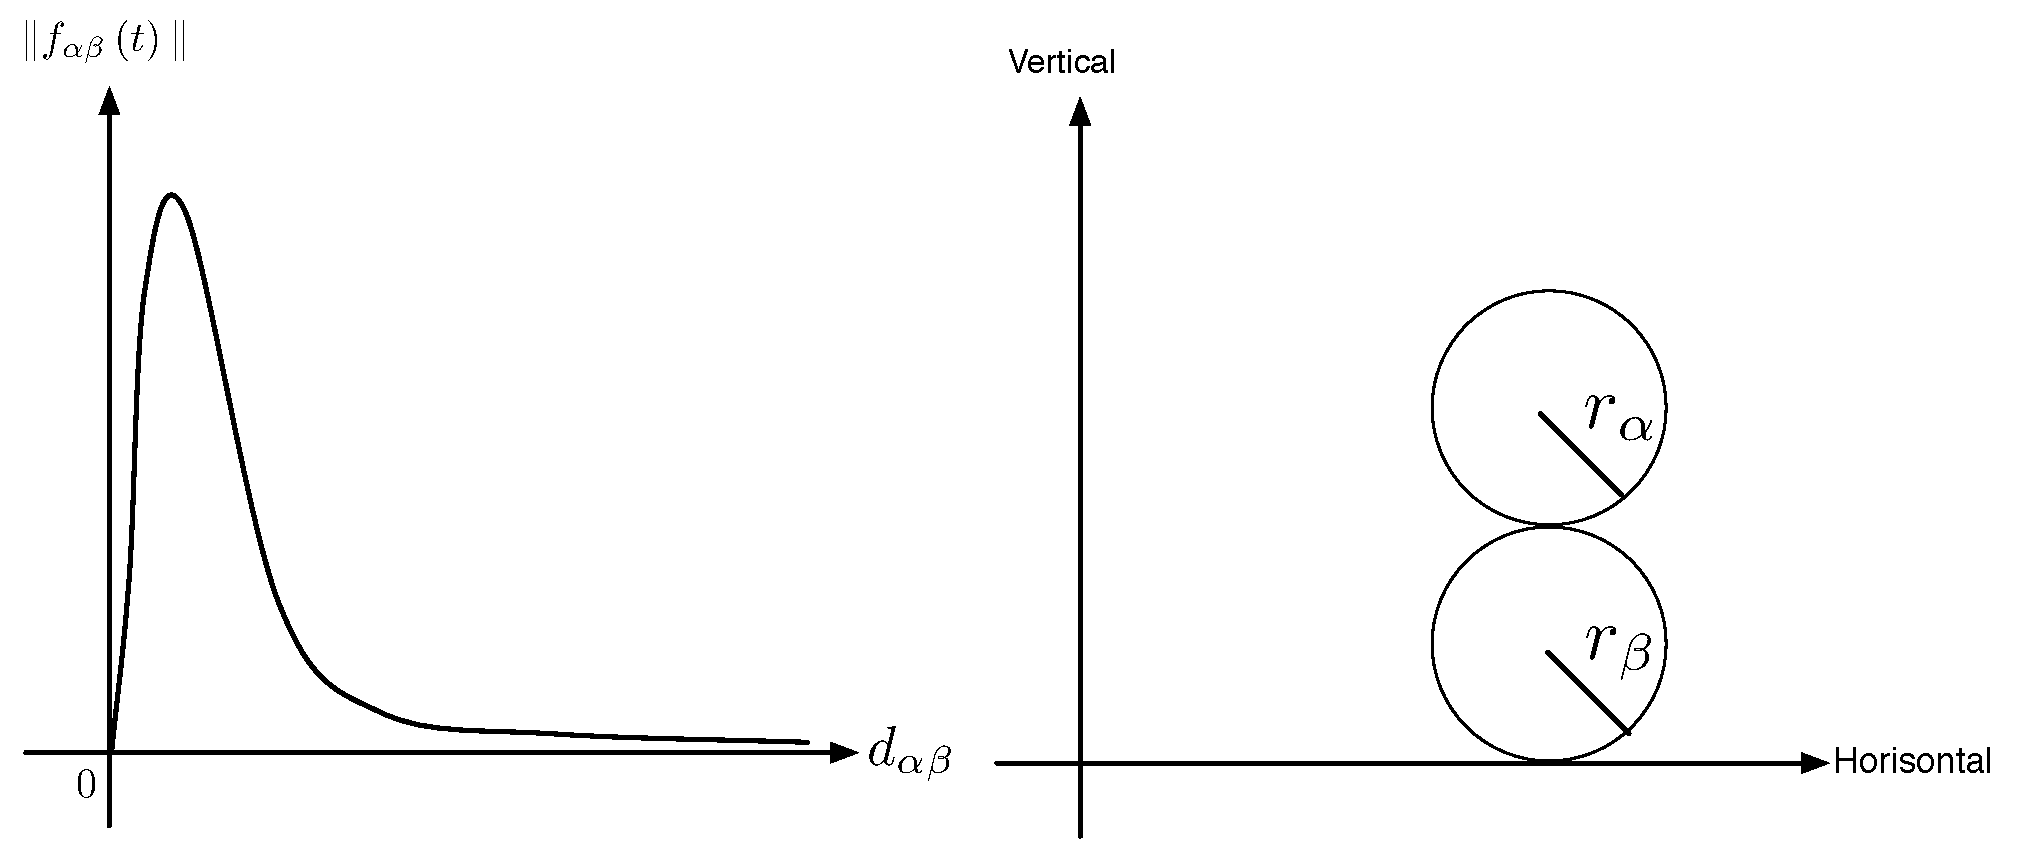
\includegraphics[scale=0.35]{Figures/ForceOverlapping.pdf}} 
    \caption{}
    \label{forceoverlapping}
\end{figure}
 
\subsection{Tangential forces}
Here we discuss the idea of improving the model by improving tangential forces, that is, the force parallel to the surface of an object.
The tangential forces can be used as collision avoidance, so that agents steer around obstacles or other agents \cite{tang}.
This would be relevant when simulating an environment where, e. g., and is standing in the middle of a symmetrical room and the agent's waypoint
is behind a big square pillar, with equal distance either way around, the agent would get stuck in front of the pillar without the tangential forces,
since the forces acting on the agent's motivation is cancelling each other out. 
In our case where two groups of agents are crossing each other in a corridor, the tangential force would make the agents to into account
the position of the agents in front of them and steer around them.

The tangential forces can also improve the model so it can simulate agents escaping a smoke filled room where we determine the visibility.
In this case of simulation the agents would walk randomly around untill they find a wall, and follow the wall around due to the tangential force.
This would be a way of implementing way finding to the model.

Friction between agents would also be possible to add to the model, since the tangential forces from other agents would make it
harder for agents to walk through a crowd. \cite{self-org} mention that friction is causing clogging in front of exits, since the people
get stuck in each other. In our simulation the agents are not clogging as heavily as \cite{self-org} mention it can be.
The time it take for the agent to leave a room in unrealistic low, and we think that implementing the friction by tangential forces
would make the simulation time more realistic.
